\documentclass%[review]
              {elsarticle}
\usepackage[utf8]{inputenc}
\usepackage{hyperref}
\usepackage{listings}
\usepackage{color}
\usepackage{xspace}

%\usepackage{lineno}
%\modulolinenumbers[5]
%\linenumbers

\lstdefinestyle{customc}{
  language=C,
  basicstyle=\scriptsize,
  backgroundcolor=\color{white},
  frame=single,
  captionpos=b,
  morekeywords={int64_t, int32_t}
}

\lstdefinestyle{BOAST}{
  language=Ruby, 
  basicstyle=\scriptsize, 
  backgroundcolor=\color{white}, 
  frame=single, 
  captionpos=b,
  morekeywords={BOAST, pr, decl, opn, close}
}

\lstdefinestyle{customf}{
  language=FORTRAN,
  basicstyle=\scriptsize,
  backgroundcolor=\color{white},
  frame=single,
  captionpos=b
}

\usepackage{url}

\journal{Journal of Parallel and Distributed Computing}

%%%%%%%%%%%%%%%%%%%%%%%
%% Elsevier bibliography styles
%%%%%%%%%%%%%%%%%%%%%%%
%% To change the style, put a % in front of the second line of the current style and
%% remove the % from the second line of the style you would like to use.
%%%%%%%%%%%%%%%%%%%%%%%

%% Numbered
%\bibliographystyle{model1-num-names}

%% Numbered without titles
%\bibliographystyle{model1a-num-names}

%% Harvard
%\bibliographystyle{model2-names.bst}\biboptions{authoryear}

%% Vancouver numbered
%\usepackage{numcompress}\bibliographystyle{model3-num-names}

%% Vancouver name/year
%\usepackage{numcompress}\bibliographystyle{model4-names}\biboptions{authoryear}

%% APA style
%\bibliographystyle{model5-names}\biboptions{authoryear}

%% AMA style
%\usepackage{numcompress}\bibliographystyle{model6-num-names}

%% `Elsevier LaTeX' style
\bibliographystyle{elsarticle-num}
%%%%%%%%%%%%%%%%%%%%%%%

\begin{document}

\begin{frontmatter}

\title{BOAST: a Metaprogramming Framework to Produce Portable and Efficient Computing Kernels for HPC Applications}

%% or include affiliations in footnotes:
\author[mymainaddress]{Brice Videau}
\ead{brice.videau@imag.fr}
\author{Kevin Pouget}
\author{Luigi Genovese}
\author{Thierry Deutsch}
\author{Dimitri Komatitsch}
\author{Jean-François Méhaut}

\address[mymainaddress]{LIG/CNRS}

\begin{abstract}
The Abstract.
\end{abstract}

\begin{keyword}
Code Generation \sep Portability \sep Genericity \sep Productivity and Software
Design \sep High Performance Computing \sep Autotuning \sep Non Regression
Testing
\end{keyword}

\end{frontmatter}


\section{Introduction}

Porting and tuning HPC applications to new platforms is tedious and costly in
term of human resources.

Portability efforts are often lost when migrating to a new architecture, or code
lose maintainability because several versions of the code coexist, usually with
a lot of duplication.

Thus productivity of porting and tuning efforts is low as a huge fraction of
those developments are never used after the platform they were intended for is
decommissioned.

Genericity of HPC codes is often limited. Producing generic code in FORTRAN
90/95 is difficult as the language is not really  fit for it.

Functionality of HPC codes is tied to the previous point. Without genericity,
adding new functionalities can be quite costly.

\section{Background and Motivation}



  \subsection{Evolution of HPC Architectures}

Evolution of HPC Architectures is rapid and also diverse: in the last 5
years no less than 6 architectures have been number one in the Top500:
\begin{itemize}
\item Intel Processor + Xeon Phi (Tianhe-2)
\item AMD Processor + NVIDIA GPU (Titan)
\item IBM BlueGene/Q (Sequoia)
\item Fujitsu SPARC64 (K computer)
\item Intel Processor + NVIDIA GPU (Tianhe-1)
\item AMD Processor (Jaguar)
\end{itemize}
Being able to efficiently use those architectures on such a small
time-frame is challenging. Stress frequency of architecture changes.

The race to exascale is not going to simplify the environment. All of the above
architectures can be considered. Network architectures are also part of the
architecture and can be very diverse.  For instance European FP7 project DEEP
considers using Accelerators (XEON Phi) while the European FP7 project
Mont-Blanc considers using low-power embedded processor with integrated GPU.

Running existing applications on those new architectures is an open project.
Thus, those projects have work packages dedicated to applications. Those
workpackages are dedicated to porting and optimizing Scientific applications on
those new architectures. In the DEEP project six applications were selected for
porting and optimizing, eleven were selected in the Mont-Blanc project.
 
  \subsection{Scientific Computing Applications}

Developed by physicist, chemist, meteorologist. Usually in FORTRAN for
historical and performance reason. Codes can be quite huge (several
thousands lines of code) with lots of functionalities. Nonetheless they are
usually based on computing kernels. Computing kernels are resource
intensive and well defined parts of a program with a limited set of input
and output. Those kernels are the time consuming part of an HPC
application. They are thus the prime target for optimization.

Those applications are often developed by several individuals. Sometimes some of
those developers only work a few month on the application. Maintaining optimized
code written by someone else is quite a challenge.

In Section~\ref{use_cases} we will present two HPC application that we used
as use cases: SPECFEM3D and BigDFT. They are both based on computing
kernels and were selected as candidate applications in the Mont-Blanc project.

  \subsection{How Should Computing Kernels be Written?}

The problematic here is to obtain computing kernels that present good
performances on the architectures encountered by the application while still
being portable after the optimization process took place. Indeed the application
might encounter one of the other architectures presented before. Investing
manpower to optimize the application for a new architecture is reasonable,
suffering hindrance from previous optimization work is not. Thus optimizations
have to be as orthogonal as possible from one another so as to be easily
activated and deactivated.

If this paradigm is followed by developers then they will rapidly be confronted
with a huge optimization space to search. They will need to be able to test
easily the performance impact of the chosen optimizations without running the
full application. The same reasoning implies that kernels should be tested for
non regression without running the full application.

What we want is computing kernels that are:
\begin{itemize}
\item Written in a \emph{portable} manner,
\item Written in a way that raise developer \emph{productivity},
\item Written to present good \emph{performance}.
\end{itemize}

\section{BOAST: Using Code Generation in Application Autotuning}

\begin{figure}
\begin{center}
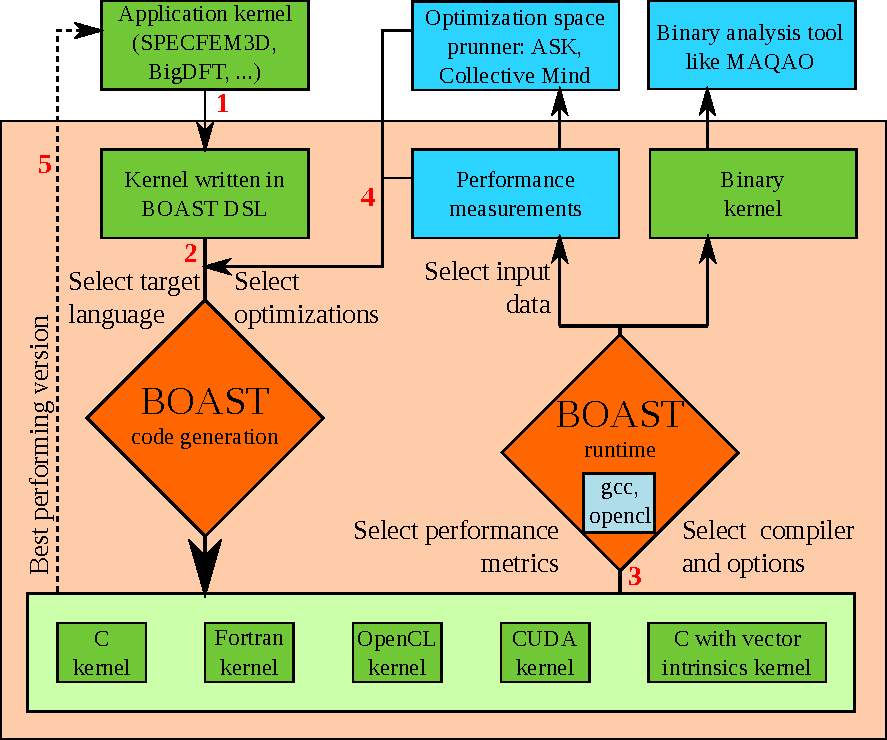
\includegraphics[width=\textwidth]{BOAST_Workflow.pdf}
\caption{Structure and Workflow of the BOAST framework.}
\label{fig:boast_workflow}
\end{center}
\end{figure}

  The idea behind BOAST is to provide scientific application developers with a
framework to develop and test application computing kernels. The envisioned
workflow and program structure is presented in Figure~\ref{fig:boast_workflow}.
The user should start from an application kernel (implemented or just designed)
and implement it in a dedicated language (step 1). The language provides enough
flexibility for the kernel to be meta-programmed with several orthogonal
optimizations. Then the developer selects one configuration of the kernel and a
target language. Those parameter define the output source code that will be
generated by BOAST (step 2). The resulting code source is then built according to
the user specified compiler and options (step 3). If input data are available
then the kernel can be benchmarked and tested for non regression. Based on the
results, other optimizations can be selected (step 4) or new optimizations can
be added to the BOAST sources. The process can be repeated until a good
candidate is found on the target platform. The resulting kernel is then added to
the program (step 5).

Several of the steps in the workflow can be automated: optimization and compiler
flags exploration, non regression testing, benchmarking... This automation can
be done by scripting by the user or by interfacing other dedicated tools. In
order to achieve those goals three aspects should be considered:
\begin{itemize}
\item code description,
\item code generation,
\item and kernel execution runtime.
\end{itemize}

  \cite{videau2013boast}

  \subsection{Kernel Description Language}

  \begin{itemize}
  \item Abstraction of programming concepts: variables, procedures (
portability, productivity )
  \item Operator overloading: simpler syntax ( productivity, portability )
  \item Two languages in one ( productivity, performance ) 
  \end{itemize}

Usually computing kernels are hotspots of an HPC application, and are most of
the time based on a loop nest. A lot of effort is dedicated to their tuning and
the obtained result is often quite different than the original procedure.
Several transformations can be applied to such kernels. And those optimization
are often applied manually as compiler may fail to recognise the opportunity.

There are many different loop optimization techniques~\cite{wolf1991loop}. We
can cite loop skewing~\cite{wolfe1986loops} (derives nested loops wavefronts)
or loop interchange~\cite{allen1984automatic} (loop variables change places).

The importance of  correct loop imbrication on BLAS~\cite{lawson1979basic}
operations is studied in~\cite{soliman2009performance}, and shows performance
increase of a factor up to 5 when using correct loop imbrication. The importance
of code transformation is stressed in~\cite{ye2011porting}, where a selection of GPU
kernels are ported to CPU and optimized.

BOAST kernel description language should be able to express all these
optimizations. This gives us a set of constraints to implement in the language:
\begin{itemize}
\item Arbitrary number of variables have to be created and manipulated (types,
attributes...).
\item Procedures have to be abstracted (reunite FORTRAN and C like languages,
attributes...).
\item Functions must be available.
\item Variables, constants and functions must be composed in complex
Expressions.
\item Basic control structures (for, while, if/else...) have to be abstracted.
\item Powerful array management (several dimensions, transformations,
indexing...).
\end{itemize}

\begin{figure}
\begin{center}
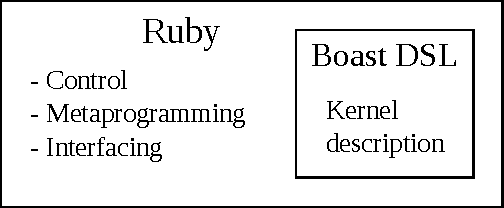
\includegraphics[scale=0.8]{BOAST_DSL.pdf}
\caption{BOAST DSL intent.}
\label{fig:dsl}
\end{center}
\end{figure}

In order to manipulate those abstractions we want to have a syntax resembling
what programmers use. For instance commonly used operator have to be available
and behave as expected. It must also be possible to differentiate an action on
an abstraction in the context of an expression and in the context of the
management of this expression. This is why an embedded domain specific language
approach was selected~\cite{hudak1996building}. This allows for the coexistence
of two languages: the host language and the DSL. In our case the DSL allows the
description of the kernel while the host language provides the meta programming
of the kernel, cf Figure~\ref{fig:dsl}. Operator overloading of the host
language will provide the familiar syntax programmers are accustomed to.

It was also important to have our constructs like \emph{for} loops to have a
syntax approaching those commonly found in programming languages. For this we
needed a language which could seamlessly pass a block of code to a function.
Ruby~\cite{matsumoto2002ruby} is one such language. It has deep introspection
capabilities as well. This is the main reason it was selected.

    \subsubsection{BOAST keywords}


In order to clearly differentiate what is going to be generated from what is
related to manipulations in the host language four keywords were defined. They
are \emph{pr}, \emph{decl}, \emph{opn} and \emph{close}. As the language is
an EDSL, these four keywords are methods in the BOAST namespace.

The \emph{pr} method calls the public \emph{pr} method of Objects it is
called on. Each BOAST object is responsible for printing itself correctly
depending on the BOAST configuration at the time the print public method is
called. Calling directly the print method of a BOAST object yields the same
result.

The \emph{decl} method is used to declare variables or procedures and functions.

The \emph{opn} method can be used to print the beginning of a control
structure without an associated code block.

The \emph{close} method is the counterpart to the \emph{opn} method. It is used
to close a control structure without an associated code block.

    \subsubsection{BOAST Abstractions}

BOAST defines several class that are used to represent the structure of the
code. These classes can be sorted in two groups, algebraic related and control
flow related:

      \paragraph{Algebra}

\begin{figure}
\lstset{style=BOAST,
        caption={BOAST code}, 
        label={lst:BOAST_algebra},
        numbers=left }
\begin{lstlisting}
i = BOAST::Int("i") # or BOAST::Variable::new("i", Int)
k = BOAST::Int("k", :size => 8)
l = BOAST::Real("l", :dim => [ BOAST::Dim(-5, 21) ], :local => true )
BOAST::decl i, k, l
BOAST::pr i === 5
j = i + 5
BOAST::pr k === j * 2
BOAST::pr l[k] === 1.0
BOAST::register_funccall("sin")
BOAST::pr l[k+1] === BOAST::sin(j)
\end{lstlisting}

\begin{minipage}[b]{0.50\linewidth}
\centering
\lstset{style=customf,
        caption={FORTRAN output.},
        label={lst:BOAST_algebra_FORTRAN} }

\begin{lstlisting}
integer(kind=4) :: i
integer(kind=8) :: k
real(kind=8), dimension(-5:21) :: l
i = 5
k = (i + 5) * (2)
l(k) = 1.0_wp
l(k + 1) = sin(i + 5)
\end{lstlisting}
\end{minipage}
\hspace{0.04\linewidth}
\begin{minipage}[b]{0.44\linewidth}
\centering
\lstset{style=customc,
        caption={C output.},
        label={lst:BOAST_algebra_C} }

\begin{lstlisting}
int32_t i;
int64_t k;
double l[27];
i = 5;
k = (i + 5) * (2);
l[k - (-5)] = 1.0;
l[k + 1 - (-5)] = sin(i + 5);
\end{lstlisting}
\end{minipage}
\caption{BOAST Code Snippet for Variables and Expressions}
\label{fig:BOAST_algebra}
\end{figure}
The first and most fundamental abstraction is named Variable. Variables have a
type, a name and a set of named attributes. The existing attributes are mainly
inspired from FORTRAN. Those attributes are not limited and can be arbitrarily
enriched, allowing a lot of flexibility in Variable management.

The second abstraction is named Expression. It is used to combine variables into
algebraic or logic expressions. Most of the classical operators are overloaded
for those two abstractions and thus the syntax of the expressions are rather
straightforward. The exception is the assignment operator as it is important to
differentiate between assigning an Expression or a Variable in the ruby context
and the assignment operator in the context of a BOAST Expression. Thus the
assignment in a BOAST Expression is represented as the \emph{===} operator,
while the classical assignment is kept as the \emph{=} operator. Function calls
(FuncCall) are also abstracted and can be used in Expressions.

Figure~\ref{fig:BOAST_algebra} shows some basic usage of both Variables and
Expressions as well as the \emph{pr} and \emph{decl} keywords. For clarity we
stayed out of BOAST namespace so BOAST related class and methods are prefixed
with \emph{BOAST::}. Listing~\ref{lst:BOAST_algebra} shows the BOAST code that
when run produces the FORTRAN (Listing~\ref{lst:BOAST_algebra_FORTRAN}) and C
(Listing~\ref{lst:BOAST_algebra_C}) output. At first we define 2 Variables
\emph{i} and \emph{k} (note that \emph{k} is $64$ bit integer). The third variable
named \emph{l} is a one dimensional local array of a length of $27$, it is indexed
in the range $-5$ to $21$. All those Variables are affected to ruby variables
of the corresponding name.

On Line~4 we declare those three variables. Variable \emph{i} is then affected
the value 5. On Line~6 the \emph{j} ruby variable is used to store the BOAST
expression \emph{$i+5$}. This variable will the be used transparently through
the rest of the program.

On Line~8 we use the \emph{k} variable to index into the array \emph{l} using
the bracket operator. Would the array be multidimensional the index would be
coma separated, similar to FORTRAN notation.

On the last line, a call to the \emph{sin} function is made through the creation
of a FuncCall object.  The possibility to use this method is declared using the
\emph{register\_funccall} method.

      \paragraph{Control Structures}

\begin{figure}
\lstset{style=BOAST,
        caption={BOAST code}, 
        label={lst:BOAST_control},
        numbers=left }
\begin{lstlisting}
BOAST::register_funccall("modulo")
i = BOAST::Int("i")
j = BOAST::Int("j")
BOAST::pr j === 0
BOAST::pr BOAST::For( i, 0, 100 ) {
  BOAST::pr BOAST::If( BOAST::modulo(i,7) == 0 ) {
    BOAST::pr j === j + 1
  }
}
\end{lstlisting}

\begin{minipage}[b]{0.47\linewidth}
\centering
\lstset{style=customf,
        caption={FORTRAN output.},
        label={lst:BOAST_control_FORTRAN} }

\begin{lstlisting}
j = 0
do i = 0, 100, 1
  if (modulo(i, 7) == 0) then
    j = j + 1
  end if
end do
\end{lstlisting}
\end{minipage}
\hspace{0.04\linewidth}
\begin{minipage}[b]{0.47\linewidth}
\centering
\lstset{style=customc,
        caption={C output.},
        label={lst:BOAST_control_C} }

\begin{lstlisting}
j = 0;
for (i = 0; i <= 100; i += 1) {
  if (modulo(i, 7) == 0) {
    j = j + 1;
  }
}
\end{lstlisting}
\end{minipage}
\caption{BOAST Code Snippet for control structures}
\label{fig:BOAST_control}
\end{figure}

The classical control structures are implemented. \emph{If}, \emph{For},
\emph{While}, \emph{Case} are abstractions in BOAST matching the behavior of
corresponding control structures in other languages. An exception is the For in
BOAST more closely matches the for in FORTRAN than the one in C.

Figure~\ref{fig:BOAST_control} show some basic usage of the control structures.
The example a C macro or function that behaves similarly to the FORTRAN modulo
intrinsic. The sample script (inefficiently) computes and stores in \emph{j} the
number of multiples of $7$ in the 0 to 100 range. It uses the For and If control
structures. A Ruby block is passed to each of those constructs. This block is
evaluated at the time the construct is printed. If several such constructs are
needed (in an \emph{if elsif else} case for instance) they can be explicitly
passed as parameters using the \emph{lambda} Ruby keyword.

\begin{figure}
\lstset{style=BOAST,
        caption={BOAST code}, 
        label={lst:BOAST_procedure},
        numbers=left }
\begin{lstlisting}
n = Int("n", :dir => :in)
ndat = Int("ndat", :dir => :in)
x = Real("x", :dir => :in, :dim => [ Dim(0, n-1), Dim(ndat) ])
y = Real("y", :dir => :out, :dim => [ Dim(ndat), Dim(0, n-1) ])
p = Procedure("magicfilter", [n, ndat, x, y])
opn p
close p
\end{lstlisting}

\lstset{style=customf,
        caption={FORTRAN output.},
        label={lst:BOAST_procedure_FORTRAN} }

\begin{lstlisting}
SUBROUTINE magicfilter(n, ndat, x, y)
  integer(kind=4), intent(in) :: n
  integer(kind=4), intent(in) :: ndat
  real(kind=8), intent(in), dimension(0:n - (1), ndat) :: x
  real(kind=8), intent(out), dimension(ndat, 0:n - (1)) :: y
END SUBROUTINE magicfilter
\end{lstlisting}
\lstset{style=customc,
        caption={C output.},
        label={lst:BOAST_procedure_C} }

\begin{lstlisting}
void magicfilter(const int32_t n, const int32_t ndat,
                 const double * x, double * y)
}
\end{lstlisting}
\caption{BOAST Code Snippet for Procedure}
\label{fig:BOAST_procedure}
\end{figure}

The last control structure is Procedure. It is used to describe either procedure
or functions. Figure~\ref{fig:BOAST_procedure} presents the use of this
abstraction. It is the signature of a real kernel from BigDFT. This kernel uses
an input array \emph{x} and an output array \emph{y} of double precision
numbers. Those array have two dimensions which depend on input variables
\emph{n} and \emph{ndat}. We can see here the use of the \emph{opn} and
\emph{close} keywords that are used to print a control structure without an
associated Ruby block. This time we placed ourselves inside of BOAST namespace.

The generated outputs in FORTRAN~\ref{lst:BOAST_procedure_FORTRAN} and
C~\ref{lst:BOAST_procedure_C} show the difference in meta-information that is
kept between both versions.
  
%Considering source-to-source transformations that we investigate with the BOAST
%tool in this paper, we can compare ourselves to POET~\cite{POET2012}  and
%ABCLibScript~\cite{ABCLib2006}. However, both tools apply transformations
%to the syntaxic tree of a program while BOAST intervenes well before in the
%transformation process. Indeed, one may first use BOAST on order to generate a
%program (a specific syntactic tree) and then benefit from the transformation
%facilities offered by one of the above tools.

  \subsection{BOAST Runtime}

In the previous Section we presented BOAST's language. This allows us to
describe procedures and functions and to meta-program them using Ruby. But in
order to find the best version of a computing kernel each version has to be
compiled, linked and then executed to assess it's performance. This can be very
time consuming if this process cannot be automated. By enabling more versions to
be evaluated the automation will bring improved portability, better performance
and in the end improve the productivity of the developer.

In this section we will present the different aspects of BOAST runtime that
allow this automation. Those aspects are listed here:
  \begin{itemize}
  \item multi target language generation ( performance, portability )
  \item compilation ( productivity, performance )
  \item execution ( productivity, performance )
  \item tracer, dumper and replay for non regression tests ( productivity )
  \end{itemize}

  \subsubsection{Multi-target Language Generation}

Language availability and performance can vary between platforms. It is thus
important to be able to express computing kernels in different languages, based
on the availability and their respective merits on the target platform. Some
languages can have additional features, such as languages that target GPUs
(OpenCL, CUDA). The developer should be given tools to determine what kind of
language is currently used in order to be able to use those additional features.

Similarly the target language must be changed with ease in order to compare
different alternatives. Two methods are dedicated to this task: \emph{set\_lang}
and \emph{get\_lang}. The target language can also be set through environment
variable before launching BOAST, allowing for easy command line scripting.

  \subsubsection{Compilation}

Compilation of the generated kernels must also be very flexible. Indeed, HPC
applications may encounter platforms with very diverse compilation environment.
Proprietary and dedicated compilers are common on HPC infrastructures. Thus
BOAST build system shows similar behavior than common build system. Compilers
and their compile/build options can be specified. This can be done at several
places. Here is the list by increasing order of precedence: BOAST configuration
file, environment variables and at kernel build time.

This way the framework to test different compiler optimizations is completely
available and performance study can include both kernel related parameters and
compilation related parameters. This behavior is contained in the \emph{CKernel}
class of BOAST. When instantiating this class a BOAST \emph{Procedure}
representing the entry point of the kernel is specified.

  \subsubsection{Execution}

The next logical step is to benchmark the built kernel. Boast offers a simple
way to run a kernel that was successfully built while staying inside of BOAST.
A built BOAST \emph{CKernel} exposes a run method that accepts arguments corresponding
to the BOAST \emph{Procedure} used to instantiate the kernel. Arrays must be
instances of \emph{NArray} which are numerical arrays that use C array
underneath.

Arrays which correspond to output parameters will be modified during the
execution of the kernel so results can be checked. This allows for easy non
regression testing. The run method also returns information (and result for
kernels that are functions) about the run. For instance the run time of the
kernel is one such information, it is obtained using the system wide realtime
clock. Other probes can be inserted at compile time if needed.

  \subsubsection{Kernel Replay}

The non regression methodology presented before is viable provided input data
can be generated at runtime. Unfortunately it is not always possible, some
applications have very complicated data patterns that are difficult to
synthesize without running the full application. Thus BOAST offers a way to load
binary data from the file system and use them as inputs of a kernel. Outputs can
also be checked against those binary data thus enabling (almost) data oblivious
non regression testing.

In order to use this methodology one has to be able to trace an application to
get input data. Such a tracer, dedicated to CUDA and OpenCL, will be presented
in the SPECFEM3D use case.

\section{Use Cases}
\label{use_cases}

  \subsection{Creating an Auto-Tuned Convolution Library for BigDFT using BOAST}

    \subsubsection{BigDFT}

BigDFT~\cite{bigdft} is a scientific application computing the electronic
structure of systems using density functional
theory (DFT). The application is mainly written in Fortran and currently
includes some 193,000 lines of Fortran code, which accounts for more than 50 \% 
of the code base. It is a parallel application based on the standards
MPI~\cite{mpi} and OpenMP~\cite{openmp}.  It also supports CUDA~\cite{cuda} and
OpenCL~\cite{opencl}.  As it is used on systems that may
have very different architectures, it is of great importance to be able to
optimize and run the application according to the specific underlying platform.


BigDFT is characterized by its extensive use of
convolution operators~\cite{nussbaumer1982fast} applied on large arrays of
data.  One example of a specific convolution, called
MagicFilter~\cite{Genovese|CAS2010}, can be seen in Listing~\ref{lst:conv_example}. 
It applies a filter $filt$ to the data set $in$ and then stores the result in the data set $out$ with a
transposition~\cite{Goedecker1993}.

\lstset{	language=C, 
		basicstyle=\scriptsize, 
		backgroundcolor=\color{white}, 
		frame=single, 
		captionpos=b,
		caption={MagicFilter}, 
		label={lst:conv_example}}
		
\begin{lstlisting}
double filt[16] = {F0, F1, ... , F15};
void magicfilter(int n, int ndat, double* in, double* out){
  double temp;
  int m;
  for( j = 0; j < ndat; j++) {
    for( i = 0; i < n; i++) {
      temp = 0;
      for( k = 0; k < 16; k++) {
        m = (i-7+k)%n
        temp += in[m + j*n] * filt[k];
      }
      out [j + i*ndat] = temp ;
    } 
  }
} 
\end{lstlisting}

As we can see, there are three nested loops working on arrays whose sizes
vary.  Various optimizations can be applied to this treatment and
may focus on the loop structure, as well as on the size of the data.  In this
paper we focus on this particular convolution and explore different
optimizations whose nature is presented in detail in the next section.

    \subsubsection{A Generic Convolution Library}

  BigDFT implementation of convolution/wavelets is a reference but is limited in scope (1 wavelet family ands its derived operators).
  Generalizing to other wavelet families long and difficult if performance are to remain good.

Idea:
\begin{itemize}
\item write a generic convolution library in BOAST
\item BLAS like interface
\item Provide a wide variety of building blocks
\item Optimize thos blocks using BOAST
\item Build either from source or directly link with binary
\item Release complete library
\end{itemize}


  Characteristic use case driven

  Convolution Library: first step toward a dsl dedicated to wavelet processing for Physics computing.
  
\newcommand{\productname}[1]{\textsc{#1}}
\newcommand{\latin}[1]{\textit{#1}}

\newcommand{\Specfem}{\productname{Specfem 3D}\xspace}
\newcommand{\Cuda}{\productname{Cuda}\xspace}
\newcommand{\eg}{\latin{e.g.,}\xspace}
\newcommand{\OCL}{\productname{OpenCL}\xspace}
\newcommand{\code}[1]{\texttt{#1}}

\newcommand{\etc}[1]{\latin{etc}}


\subsection{Porting SPECFEM3D to OpenCL using BOAST}
\label{subsec:specfem}

\subsubsection{SPECFEM3D}

In this last subsection, we study a free seismic wave propagation
simulator, \Specfem, in its \productname{Cartesian}
flavor\footnote{Specfem3d Cartesian --- CIG
  \url{http://www.geodynamics.org/cig/software/specfem3d}}. \Specfem
simulates seismic wave propagation at the local or regional scale
based upon spectral-element method (SEM), with very good accuracy and
convergence properties. ADD BENCHMARK APP FOR HPC SUPERCOMPUTERS.

When we started to work on the project (version v2.1 of July 2013) it
supported graphics card GPU acceleration through NVidia \Cuda. This
GPU support comes in addition to the MPI support implemented to enable
parallel computing. Most of \Specfem code-base is written in
\productname{Fortran2003}, only the GPU related parts are written in
C.  The split between CPU and GPU code was done at a rather fine
grain, as the application counted more than 40 GPU kernels. Some of
them were quite simple (\eg performing a few vector operations, but at
massively parallel scale), while at the other side of the spectrum,
some complex kernels took more than 80 parameters and perform very
specific physical transformations.

Because of the complexity of wave propagation (and of the application
architecture), it is hard to impossible to define unit tests. Hence,
the application is validated by the accuracy of the results it
produces, that is, the accuracy of seismograms of the simulated
earthquakes, in comparison with the actual ones. Non-regression
testing (after new developments) is also based on these seismograms,
with measurements of the relative error between two identical
simulations.

As part of the Mont-Blanc project, we had to port \Specfem to \OCL, so
that it could be use to benchmark Mont-Blanc HPC platforms.

\subsubsection{Porting to OpenCL}

\subparagraph{Porting kernels to BOAST} Nvidia \Cuda and \OCL are
based on the \emph{same} programming model: a massively parallel
accelerator running in a distinct memory environment. Thanks to that
proximity, we, BOAST developers, have been able to carry out most of
the porting task with only a limited knowledge about \Specfem internal
physics.

That lack of knowledge led us to be particularly attentive to the path
we undertook for the porting, as we would have been unable to
understand how and why the application was not operating properly, if
it was to fail.

Hence, our first milestone in the porting was translating \Specfem
\Cuda kernels to BOAST EDSL. This way, we could ask BOAST framework to
generate CUDA versions of the kernels, plug them back into \Specfem and
get (after fixing compile-time errors---prototypes and naming mistakes
mainly) a first set of \Specfem seismograms.

As we had expected, the seismograms were erroneous. But with the help
of shell scripts and BOAST framework ability to store and provide the
kernels' original source code, we built a set of \Specfem binaries
including only \emph{one} BOAST-generated kernel, with all others
reference-kernels. Running and validating all these binaries enabled
use to pinpoint the misbehaving kernels. We finished the debugging
with a side-by-side comparison that highlighted the coding mistakes.

\subparagraph{Porting runtime to \OCL} The second part of the porting
consisted in translating the CPU-side of the application from \Cuda
API to \OCL API. Most of the functions of the interfaces are very
similar, with only naming-convention and data-structure
distinctions. Hence, it was clear that automatic rewriting tools
(namely \code{sed} regexp and \code{emacs-list} functions) could be
useful. To give an idea of the cost of a \emph{manual} rewriting, we
can count (in \# of \OCL API function calls): 70 kernel ``function
calls'', 790 arguments to set, 230 memory transfers, 160 buffer
creations and 270 releases.

Once all the automatic (and many manual) transformations applied,
compilation errors fixed, and \OCL unsuccessful function calls solved,
the application managed to complete its execution and generated a
first set of seismograms. And again, as expected and feared, these
seismograms were not valid.

As we had already validated BOAST-generated kernels (and trusted \Cuda
and \OCL versions to be semantically identical), we knew that the bugs
were now in the CPU side, and we had to find a way to understand where
\Specfem's \Cuda version of the code diverged from its \OCL
counterpart. To help us in that purpose, we had a strong assumption:
both versions of the code were supposed to perform exactly the same
operations, with the same ``logical'' parameters (the APIs have
\emph{implementation} differences, for instance \OCL has two memory
transfer functions, \code{clEnqueueReadBuffer},
\code{clEnqueueWriteBuffer}, whereas \Cuda has only one, with a
direction parameter \code{cudaMemcpy(..., dir)}, but above that it is
the same functionality nonetheless).

Hence, our idea to locate the execution problems was to make sure that
both execution actually did the same thing. As the \OCL results were
invalid, we knew the executions would diverge at one or several
points.

\subparagraph{Debugging \OCL Execution: \code{GPUTrace}} In order to
ensure that \Cuda and \OCL executions were doing the same operations,
we developed a tool that could intercept all the function calls
related to the GPU and store them for offline processing, in a format
common to \OCL and \Cuda. Our solution was inspired by \code{strace}
and \code{ltrace} tools: it dynamically preloads a library (with the
help \code{LD\_PRELOAD} in \productname{GNU/Linux}-based environments)
between the application and the GPU library, and prints the arguments
(input \emph{and} output) of the relevant function calls.

However, in contrast with \code{strace} and \code{ltrace},
\code{GPUTrace} has to be \emph{state-full}. Indeed, most of \OCL and
\Cuda parameters are handles to opaque types, so, in order to provide
more meaningful information, \code{GPUTrace} stores internally
information about these handles (buffer creation size and index,
kernel name and prototype, \etc). % more details here?

Once \code{GPUTrace} was operational, it was easy to confront \Cuda
and \OCL outputs with a graphical \code{diff} tool, and spot the
different porting mistakes: two parameters reversed, an offset
incorrectly applied, \etc. One last problem remained, impossible to
miss because of the seismograms not matching (but with just a slight
drift). We added more verbosity to \code{GPUTrace} output, first the
initial bits of the GPU memory buffers, then their full content. The
drift was visible in the trace, but it was nonetheless unclear where
it started. We finally got it after hours of code review, both on
BOAST kernels and \OCL code: one kernel was \emph{three}-dimensional,
whereas the others were two-dimensional. But for all of them, only two
dimensions were passed. As it was the same person who coded the \OCL
port and the GPU tracer, this third dimension was forgotten in both
side\ldots

\subparagraph{Evaluation} Our \OCL/BOAST port of \Specfem is now
merged in \Specfem's development tree and under test and extension by
different research teams. On a platform with two K40x GPUs and x Intel
Xeon processors, we measured similar results between the original
\Cuda version and our BOAST-\Cuda version. With the same set of
optimization, BOAST \Cuda and \OCL version also reported similar
execution time spans. The best execution speed (25\% higher) was
achieved with \Cuda version though, as one optimization parameter
(\code{CUDA\_LAUNCH\_BOUND}) cannot be passed, as of version 1.1, to
\OCL runtime.

By refactoring GPU kernel code in BOAST EDSL, the size of kernel code
shrank by a factor of 1.5 (from xxx LOC to xxx, in part because of
code duplication, but by removing manually unrolled loops). This is
beneficial for \Specfem as it improves the readability and
maintainability of its source code.

We have also been able to enhance \Specfem's non-regression testsuite
by adding per-kernel non-regression tests. This was done with the help
of \code{GPUTrace}, that we used to capture all the input parameters
of a particular \emph{valid} kernel execution, as well as the output
values. Then, during the non-regression testing, BOAST framework can
load these buffer files, allocate and write them on the GPU memory
through \Cuda or \OCL runtime, and trigger the kernel execution. A
comparison of the output values (for instance against a maximal error
level) validates the non-regression.

In the same mindset, we provided \Specfem testsuite with kernel
performance evaluation mechanisms. These tests will help developers to
try new optimization in kernel code and measure their impact, without
executing the whole application.

%%%%%%%%%%%%%%%%%%%%%%%%%%%%%
%%% Local Variables:      %%%
%%% mode: latex           %%%
%%% TeX-master: "journal" %%%
%%% TeX-PDF-mode: t       %%%
%%% End:                  %%%
%%%%%%%%%%%%%%%%%%%%%%%%%%%%%


\section{Related Work}

Code generation and auto-tuning techniques are not new. Nonetheless, with recent
developments in hardware, and the HPC landscape being as diverse as it is now,
there is a renewed interest in the field. This related work Section is split in
three parts, focusing first on Auto-tuning frameworks. Tools that provide a DSL
to describe computing kernels will then be presented. Last, optimization space
pruners and their ties to auto-tuning will be introduced.

  \subsection{Application Auto-Tuning} 

  The most convenient way to obtain an application that can be auto-tuned on a
given platform is to base this application on a widely used computing library.
BLAS~\cite{dongarra1990set} and LAPACK~\cite{laug} are such libraries. These
libraries are either hand tuned for selected platforms or have auto-tuned
implementations. Atlas~\cite{whaley04} is an auto-tunes implementation of
BLAS/LAPACK. ATLAS authors defined the \emph{Automated Empirical Optimization of
Software} methodology that we implemented with BOAST. Their kernel generation is
done using macro-functions in C.

  Nonetheless many applications formalism cannot be reduced to standardized
library or border on what could be considered edge cases for those libraries and
not as optimized as more general cases. Orio~\cite{Hart2009:Orio} is an
auto-tuning framework that has an approach close of that of BOAST but they are
based on an annotated DSL describing loop transformation rather than a more
generic EDSL. Halide~\cite{ragan2013halide} is an auto-tuning framework
dedicated to image processing. It can also be used to describe other
operations on memory buffers. Those two frameworks propose automated search
space exploration to find the best version of a kernel.

  \subsection{Kernel Description DSL}

  The idea to describe computing kernels using a Domain Specific Language has
already been used. SPIRAL~\cite{puschel2004spiral} is a decade old generation
framework for signal processing. It uses a proprietary DSL, SPL (signal
processing language), to describe a DSP algorithm. This DSL is then transformed
into efficient programs in high level languages like C or FORTRAN.
POET~\cite{yi2007poet} also uses a DSL to describe custom code transformations,
like loop unrolling, loop blocking and loop interchange. Those transformation
can be parametrized in order to tune the application. Orio~\cite{Hart2009:Orio}
can be compared to POET as it aims at describing possible code transformations
using a DSL. All those approaches are very different from our as they put the
emphasis on compilation techniques whereas boast relies on the user to express
the different optimizations.

  Halide~\cite{ragan2013halide} is closer in some ways to our approach as it
uses an embedded C++ DSL to describe image processing algorithm. This DSL allows
decoupling the algorithm description from its scheduling. Each pixel in the
resulting image has a completely defined dependency tree with regard to pixels
in the input image (and intermediary results). During generation, depending on
memory and computing cost some values can be recomputed rather than fetched from
memory. We used Halide to implement the \emph{magicfilter} of BigDFT, but
unfortunately results were 4 to 5 times slower than the one we obtain with
BOAST. We speculate that the three-dimensional nature of our convolutions, as
well as the filter length, can be considered edge cases in halide and quite far
from the intended target.

  \subsection{Optimization Space Pruner}

  Once auto-tuning technique are used the parameter space explodes and the
systematic sampling rapidly becomes impossible to achieve. The cost of finding
the optimal kernel parameters and environment parameters (compiler flags, used
language, ...) is rapidly prohibitive. Dedicated frameworks have been developed
to address this problem. Adaptive Sampling Kit (ASK)~\cite{castro2013adaptive}
is one such tool. It reduces the number of sample needed by creating a model of
the performances and by minimizing the number of samples needed to find the
parameters of this model. Several models and sampling techniques are
implemented.

  Collective Mind~\cite{fursin:hal-01054763} proposes similar techniques to
solve the problem but also stores and the results and complete experimental
setups in databases for future reference and reproducibility. This database
approach also enables easy parallelization of the experimental process.
Collective Mind also proposes collections of flags for many available
compilers/versions easing the exploration process.

\section{Conclusion and Future Works}


\section*{References}

\bibliography{BOAST}

\end{document}
